\section[Engenharia de software]{Engenharia de software}
Hoje em dia softwares estão presente em todos os lugares, tudo que a gente 'toca'. Softwares não se desgastam (físicamente) como hardware, mas estão sujeitos a modificações durante o seu ciclo de vida \cite{Silva_filho}. As modificações as vezes podem causar efeitos acidentais e/ou não esperados. Um software precisa de modificações conforme o tempo passa e para isso acontecer com mais tranquilidade exige a necessidade de uma documentação. Quanto melhor a documentação, mais fácil para entender, porém não significa que documentação extensa é a melhor. Para manter um bom projeto de software é necessário ter ou criar uma cultura de engenharia de software para adotar as melhores práticas. As quais que compreendem os pilares de custo, tempo de desenvolvimento e qualidade de software \cite{Silva_filho}.

No glossário de terminologia de Engenharia de Software da IEEE Std 610.12-1990, define-se Engenharia de Software como a aplicação de uma abordagem sistemática, disciplinada e quantificável para o desenvolvimento, operação e manutenção de um software; isto é aplicação de engenharia de software. Engenharia de software também pode ser o estudo das abordagens \cite{ieeeTerminology}.

Como softwares precisam de manutenção corretiva e/ou evolutiva, também está sujeito a inserção de defeitos decorrentes do desenvolvimento. Estes defeitos podem ser vistos e consertados antes da entrega \cite{Silva_filho} ou ser descoberto pelo usuário que está utilizando e não espera se deparar com o erro. Por isso além de uma documentação, software também precisa de testes, estes que quando bem feitos asseguram a qualidade e confiabilidade do produto de software.

Engenharia de software está presente e tem descrições de melhores práticas em todas as fases desde a concepção, elaboração, construção e transição de um projeto. Seja em um projeto com metologia tradicional ou ágil, um projeto passa por essas fases. A engenharia de software "tem como objetivo apoiar o desenvolvimento profissional de software, cobrindo todos os aspectos da produção de um software."\apud{monsalve}{sucessoJogoEngSoft}

[\cite{sucessoJogoEngSoft}] \cite{benittiMolleri} concordam que a engenharia de software é uma área muito jovem e sofre contínuas mudanças nos seus fundamentos tecnológicos concretizadas nos métodos e ferramentas de suporte, portanto necessita de métodos de ensino lúdicos e dinâmicos que possam contribuir na aprendizagem do estudante.


Engenharia de Software percorre o levantamento de requisitos de um jogo, o planejamento e desenvolvimento das funcionalidades, testes para garantir que está tudo funcionando como o occorido e o empacotamento e a entrega para a finalização. Após cumprir este ciclo, para um software continuar 'vivo' é necessário que com o tempo ele receba manutenção e melhorias e também se desejado, evoluções. Além de agregar valor para o cliente ou desenvolver o acordado, também é necessário gerenciar sua infra-estrutura, definir onde hospedar as aplicações, os custos decorrentes de utilizar serviços ou hardwares de terceiros, realizar as configurações para a padronização e fazer o controle de mudanças e gestão da qualidade.

\subsection[Levantamento de requisitos de software]{Levantamento de requisitos de software}
É uma das fases mais importantes. A maioria dos projetos falha pelo levantamento de requisitos incorretos. O grau de insatisfação do cliente também está relacionado à levantamento de requisitos incorretos. É importante a consolidação dos requisitos para a equipe inteira ter uma visão alinhada. A consolidação dos requisitos serve como guia para descrever as funcionalidades a serem desenvolvidas e para verificação de que o software foi construído corretamente de acordo com o esperado. Permite uma organização e maior controle do que já foi feito e está pendente para ser feito. 

\begin{comment}
\subsection[Teste de software]{Teste de software}
Teste de software é uma atividade importante do desenvolvimento de software pois está relacionado à qualidade de software, este pode ajudar a verificar o cumprimento dos requisitos.

\cite[p. 17]{Pedro_Henrique} diz que um teste tem basicamente quatro fases, o planejamento, o projeto, a execução e a avaliação do resultado dos testes. Já \cite{pressman}, \cite{delamaroJinoMaldonado} dizem que os testes devem acontecer ao longo do processo de desenvolvimento do software, pois é o momento onde as funcionalidades estão frescas no pensamento do desenvolvedor e este deve garantir com testes que ocorra o funcionamento esperando das funções.
\end{comment}

\subsection[Digital Game Based Learing LGBL]{Digital Game Based Learing LGBL}
Aplica-se em situações onde o software a ser desenvolvido é simples, os requisitos são bem conhecidos tecnologia acessível e recursos para o desenvolvimento estão disponíveis.

A metodologia Digital Game Based Learning (DGBL) é um tipo das que prezam por utilizar jogos digitais em prol do aprendizado, para isso tem que ser medido a usabilidade do software, e os resultados do jogo tem que ser efetivos.
A metodologia DGBL que continua evoluindo seu método instrucional tem a necessidade de evidências empíricas para validar seu valor educacional e mostrar como o valor poderia ser aplicado mais efetivamente \cite{jogoSuporteMat}.


Os jogos tem que ser testados em como estão sendo usado nas pessoas, pois ele podem não estar sendo benéficos. 
O autor cita que não há provas de que os jogos digitais pode sem benéficos para todas os tipos de atividades.
Com o avanço da tecnologia, os jogos complexos requerem recursos de hardware mais potente e mais tempo para jogar, o que talvez pode indicar que não deve ser usado em sala de aula, pois não substitui o repasse do conhecimento \cite{jogoSuporteMat}.


\subsection[Características dos Jogos Educacionais]{Características dos Jogos Educacionais}
Primeiramente o jogo deve motivar o jogador. Caractarísticas de jogos que atraem os jogadores, desafios, 
\cite{jogoSuporteMat} diz alguns fatores motivacionais que jogos atrativos devem ter: objetivos claros ao jogador, resultatos incertos, fornecer feedbacks e o aumento gradual de dificuldade.

Outras recomendações para os jogos educacionais é que devem estar aderidos a grandes programas educacionais e deve incorporar grandes elementos para ajudar os estudantes a construir novas estruturas de conhecimento ou completar as existentes \cite{jogoSuporteMat}.

\subsection[Plataformas mobile]{Plataformas mobile}
Existem diversas maneiras de se construir APP para mobiles. Algumas apenas para celulares Android, outras para sistemas iOS e outras para ambas plataformas. Existem \textit{frameworks} de desenvolvimento onde o código gerado já é nativo da própria plataforma alvo (Android ou iOS) e outras onde o código é transformado em partes para a plataforma nativa.
Existe um  projeto chamado \textit{kivy}, onde é escrito código na linguagem \text{Python} e o \textit{kivy} com suas bibliotecas converte o código para gerar aplicações para Android e iOS.

Outros \textit{frameworks} analisados que também geram código para ambas plataformas de celular são o \textit{Godot} e \textit{React Native}. Por maior familiaridade do autor com o \textit{HTML}, \textit{CSS} e \textit{JavaScript} optou-se por utilizar o framework \textit{React Native}.

\subsubsection[React Native]{React Native}
Aqui será explicado sucintamente o funcionamento do \textit{React Native}. O Framework trabalha com componentes e possibilita a composição e agregação de componentes. Para isso é necessário que as classes criadas extendam (herança) a classe \textit{React.Component}. Ao realizar a herança os componentes passam a ser obrigados a implementar o método \textit{render()} e também herdam dois tipos de dados: \textit{props} e \textit{states}. O método \textit{render()} faz parte do ciclo de vida da montagem e atualização de um componente é o que irá renderizar o objeto na tela mostrando a sua estilização. As props são características estáticas passadas pela classe pai que um objeto recebe ao ser criado e o state são propriedades que podem ser alteradas pelo próprio componente. Componentes extendidos da classe \textit{React.Native} passam a ter o ciclo de vida para montagem e atualização conforme descrito nas Figuras \ref{montagem} e \ref{atualizacao}.


\begin{figure}[H]
\centering
\caption{Processo de montagem do componente React}
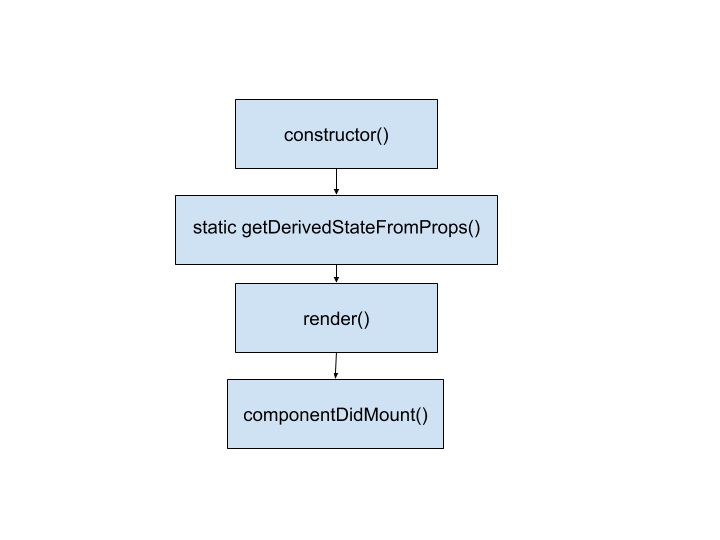
\includegraphics[scale=0.7]{figuras/montagem.png}
\label{montagem}
\\
\small{Fonte: do próprio autor}
\end{figure}

\begin{figure}[H]
\centering
\caption{Processo de atualização do componente React}
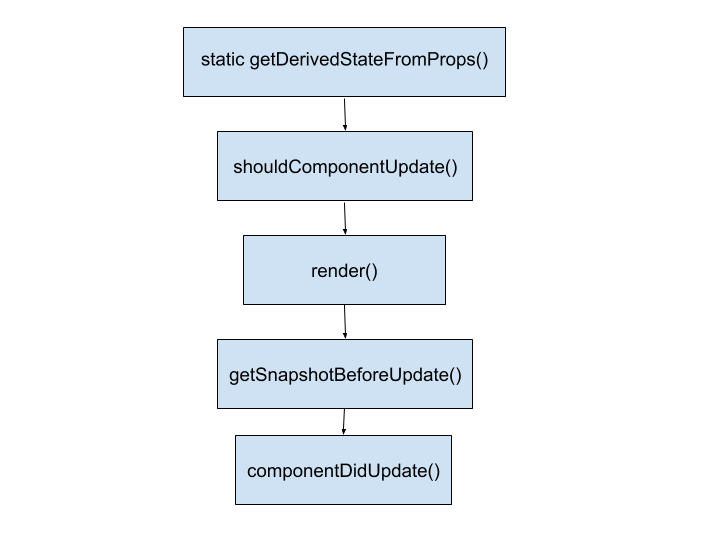
\includegraphics[scale=0.7]{figuras/atualizacao.png}
\label{atualizacao}
\\
\small{Fonte: do próprio autor}
\end{figure}
